\documentclass[11pt]{article}

\usepackage[margin=1in]{geometry}
\setlength{\headheight}{13.6pt}
\usepackage{fancyhdr}
\pagestyle{fancy}
\usepackage{scalerel}
\usepackage{mathtools}
\usepackage{amssymb}
\usepackage{xparse}
\usepackage{csquotes}
\usepackage{float}
\usepackage[inline]{enumitem}
\usepackage{circuitikz}
\usepackage{siunitx}
\usepackage{tikz}
\usetikzlibrary{arrows}
\usetikzlibrary{arrows.meta,quotes}
\usetikzlibrary{automata,positioning}

% Makes \setItemLetter work
\ExplSyntaxOn
\DeclareExpandableDocumentCommand \AlphToNum { m }
{
   \int_from_alph:n { #1 }
}
\ExplSyntaxOff

\makeatletter
% Changes the number on an \item
\newcommand\setItemNumber[1]{\setcounter{enumi}{\numexpr#1-1\relax}}
% Changes the letter on an \item
\newcommand\setItemLetter[1]{\setcounter{enum\romannumeral\enit@depth}{\numexpr\AlphToNum{#1}-1}}
\makeatother
% Aligns the top of a displaymath environment with the top of an \item
\newcommand\DisplayMathItem[1][]{%
  \ifx\relax#1\relax  \item \else \item[#1] \fi
  \abovedisplayskip=0pt\abovedisplayshortskip=0pt~\vspace*{-\baselineskip}}

\newcommand*\OR{\ |\ }

\lhead{ECE 375: Homework 1}
\chead{Jason Chen}
\rhead{January 18, 2020}

\begin{document}

\begin{enumerate}[leftmargin=0.2in]

\item
\begin{enumerate}
  \item An operation code (opcode) is a set of bits that identifies an operation that should be performed in an instruction. The size of the opcode depends on the instruction set architecture (ISA) and determines how many operations the ISA can support. The pseudo-computer from class, for example, has an ISA with 3-bit opcodes, meaning it supports $2^3$, or 8, different operations.

  \item An arithmetic logic unit (ALU) is a component that runs arithmetic and logical operations. Those would include operations such as addition, subtraction, OR, and NAND. According to the textbook, it is used for nearly all instructions, as it also performs actions like calculating effective addresses. In the pseudo-computer, the ALU takes two input values, one from the accumulator register and another from the internal data bus, and can output results back into the accumulator.

  \item An effective address is the address at which an instruction's operand(s) is stored in memory. In a direct addressing mode, the effective address of an operand would be the address provided in the instruction. However, with an indirect addressing mode, assuming only a single level of indirection, the data stored at the address in the instruction would be the actual address of the operand. That second address is the effective address. In other words, the address provided in the instruction holds a pointer to the actual operand.

  The psuedo-computer's ISA uses direct addressing, which means the address provided in the instruction is the effective address. However, it can be extended to support indirect addressing, in which case, the effective address of instruction operands is no longer the address provided in the instruction but the address stored at that memory address (assuming one level of indirection).

  \item A program counter is a register containing the address of the next instruction that should be executed. In the psuedo-computer, at the beginning of each instruction cycle (during the fetch cycle), the instruction stored at the address in the program counter is retrieved, and its opcode is sent to the instruction register, while the address of its operand is sent to the memory address register.

  \item An internal data bus is a circuit through which various components of a CPU can send data to and receive data from other components connected to the bus. In the pseudo-computer, all of the registers, along with an input to the ALU, are connected to an internal data bus, so data can be transferred between all of those components. For example, during the fetch cycle of an instruction, the program counter writes its current address to the bus, and the memory address register (MAR) reads it from the bus. At the end of the cycle, the memory data register writes the opcode and operand address to the bus, while the instruction register and MAR read the opcode and address, respectively, from the bus.
\end{enumerate}

\item A drawing of the instruction word format is below in Figure \ref{fig:q2}. The size of the opcode field is 5 bits because the CPU supports 32 instructions. Given an $n$-bit opcode, the number of possible instructions is $2^n$, so 5 bits are required for 32 instructions. The indirect addressing mode bit is only a single bit since it only has two possible states (0 or 1). Finally, the address field requires 10 bits because it must be able to address 1024 words. As with the opcodes, an $n$-bit address can refer to $2^n$ words, so 10 bits are needed to address memory with a capacity of 1K words. In total, the instruction word has 16 bits.

  \begin{figure}[H]
    \centering
    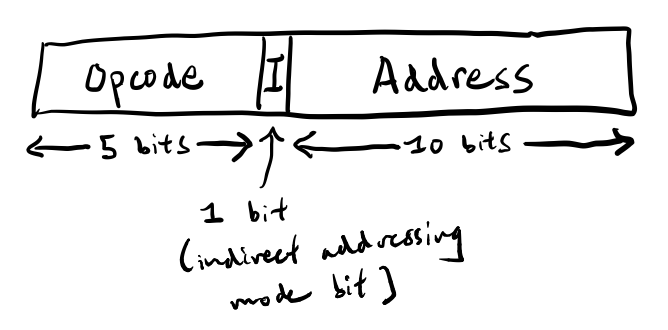
\includegraphics[width=.5\linewidth]{q2.jpeg}
    \caption{Instruction word format for question 2.}
    \label{fig:q2}
  \end{figure}

\item
\begin{enumerate}
  \item No, this operation cannot be performed in a single clock cycle because two registers cannot write to the internal data bus at the same time.

  \item This operation cannot be performed at all because IR and MAR are both smaller than MDR. IR is 4 bits, and MAR is 12 bits, but MDR contains 16 bits. To make this operation work, IR would need to only get the opcode field of MDR, while MAR gets only the address field of MDR. In that case, the operation could be performed in a single clock cycle, since the IR and MAR registers are wired to the upper four bits and lower twelve bits, respectively, of the data bus (according to Figure 3.16 in the textbook).

  \item Yes, this operation can be performed in a single clock cycle because only MDR is writing to the internal data bus, and according to pages 61-62 of the textbook, accessing memory can happen during a clock cycle, and values written to a register are not transferred into the register until the end of the clock cycle. Therefore, since accessing memory and writing into a register can happen in the same clock cycle, this operation can be performed in a single clock cycle.

  \item No, this operation cannot be performed in a single clock cycle because it requires using the ALU. From the provided picture, the ALU cannot output to the internal data bus, so there must be another transfer operation from the accumulator back into MDR. That transfer cannot happen in the same microoperation, since the result needs to be computed by the ALU first, so this operation cannot be done in a single cycle.

  \item Yes, this operation can be performed in a single clock cycle because the PC register has its own incrementer hardware, so it does not need to use the bus. Thus, MDR can write to the bus and have AC read off it, since MDR and AC are both 16 bits.

  \item No, this operation cannot be performed in a single clock cycle for the same reason that the operation in question (d) could not be performed. The operation requires use of the ALU, since PC only has incrementer hardware, so the value of PC + AC must be calculated by the ALU first and then transferred back into PC. That requires more than one microoperation, so this operation cannot be performed in a single clock cycle.
\end{enumerate}

\item
\begin{itemize}
  \item \textbf{Step 1}: MDR $\leftarrow$ M[MAR], TEMP $\leftarrow$ MAR

    In the first step, the effective address stored at address M[x] is retrieved into the MDR. Because reading data from the memory does not involve the internal data bus, the value of MAR, which is the address x, can be written to the bus and read by the TEMP register during the same clock cycle. The address x is saved into TEMP since it is used later for the post-increment after storing the accumulator.

  \item \textbf{Step 2}: MAR $\leftarrow$ MDR

    In the second step, the effective address of the operand is written into MAR, so that the accumulator can be written into that memory location (which is M[M[x]]).

  \item \textbf{Step 3}: MDR $\leftarrow$ AC

    In the third step, the current value of the accumulator is written into MDR, so that it can be written into memory location M[M[x]] in the next step.

  \item \textbf{Step 4}: M[MAR] $\leftarrow$ MDR, AC $\leftarrow$ MAR

    In the fourth step, the value of the accumulator, which has been transferred into MDR, is written to the effective address, which was placed into MAR during step 2. Simultaneously, the value of MAR is copied into AC so that it can be incremented in the next step. The currrent value of MAR is the contents of memory address x (M[X]), which is the value that needs to be incremented, according to the instruction. These two operations can be performed during the same clock cycle because writing to the memory does not involve the internal data bus. This step completes the store accumulator indirect portion of the instruction.

  \item \textbf{Step 5}: AC $\leftarrow$ AC + 1

    In the fifth step, the accumulator, which has the value M[x], is incremented in prepration for being stored back into memory location x.

  \item \textbf{Step 6}: MAR $\leftarrow$ TEMP

    In the sixth step, the original address provided in the instruction is written into MAR, since that is where the incremented address needs to be written to.

  \item \textbf{Step 7}: MDR $\leftarrow$ AC

    In the seventh step, the incremented value (M[x] + 1) in the accumulator is copied into MDR, so that it can be written into memory address x.

  \item \textbf{Step 8}: M[MAR] $\leftarrow$ MDR

    Finally, the incremented value (M[x] + 1) is written into memory location M[x], completing the post-increment part of the instruction.
\end{itemize}

\item
  \begin{enumerate}[label=(\roman*)]
  \item \texttt{ldi} loads an immediate value into a register. Register \texttt{r27} is the upper-half of the X register, and 85 is 0x55 in hexadecimal, so the contents of the X register become 0x5506.

  \item The contents of \texttt{r3} are 0x07, which is 0b00000111 in binary. \texttt{ror} shifts all bits one place to the right and shifts the carry flag into bit 7. Since the status register is 0xFF, the carry flag is 1. Thus, the binary value becomes 0b10000011, which has the hexadecimal value 0x83. Thus, the \texttt{r3} register has the value 0x83.

  \item \texttt{adc} performs addition with carry and places the result back into the first register. Because the status register is 0xFF, the carry flag is 1. The value of 0x05 + 0x1B + 1 is 0x21. Thus, the \texttt{r2} register has the value 0x21.

  \item \texttt{sts} stores the value of the register at the given data space (SRAM) location. Because there is no memory address \texttt{\$0007}, I am going to assume there is a typo and it should read \texttt{\$0107} instead. Register \texttt{r28} is the lower half of the Y register, so its value is 0x02. Thus, the contents of memory address 0x0107 are 0x02.

  \item \texttt{sbiw} subtractions an immediate value from a pair of registers. In this case, the pair of registers is the X register (XH:XL), whose value is 0x0106. The result of 0x0106 - 2 is 0x0104, so the value of the X register (XH:XL) after execution is 0x0104.
\end{enumerate}

\end{enumerate}

\end{document}
